% Created 2021-03-11 Thu 06:52
% Intended LaTeX compiler: pdflatex
\documentclass[presentation]{beamer}
\usepackage[utf8]{inputenc}
\usepackage[T1]{fontenc}
\usepackage{graphicx}
\usepackage{grffile}
\usepackage{longtable}
\usepackage{wrapfig}
\usepackage{rotating}
\usepackage[normalem]{ulem}
\usepackage{amsmath}
\usepackage{textcomp}
\usepackage{amssymb}
\usepackage{capt-of}
\usepackage{hyperref}
\RequirePackage{fancyvrb}
\DefineVerbatimEnvironment{verbatim}{Verbatim}{fontsize=\scriptsize}
\usetheme{metropolis}
\usecolortheme{}
\usefonttheme{}
\useinnertheme{}
\useoutertheme{}
\author{Petru Rebeja, Marius Apetrii}
\date{11 Martie 2021}
\title{Tehnici Avansate de Programare}
\subtitle{Gestionarea resurselor și ecosistemul NuGet}
\institute[UAIC]{Facultatea de Matematică\\Universitatea Alexandru Ioan Cuza, Iași}
\hypersetup{
 pdfauthor={Petru Rebeja, Marius Apetrii},
 pdftitle={Tehnici Avansate de Programare},
 pdfkeywords={},
 pdfsubject={},
 pdfcreator={Emacs 26.3 (Org mode 9.4.4)},
 pdflang={Romanian}}
\begin{document}

\maketitle
\section{Introducere}
\label{sec:org8410815}
\begin{frame}[label={sec:org5d6059e}]{Recapitulare}
\begin{itemize}
\item Clase abstracte vs. interfețe.
\item Acuplare și Coeziune.
\item Fluxul de lucru GitHub
\end{itemize}
\end{frame}
\begin{frame}[label={sec:org60f68bf},fragile]{Despre ce vom discuta azi}
 \begin{itemize}
\item \texttt{Garbage collector=/=IDisposable}
\item Ecosistemul \texttt{NuGet}
\end{itemize}
\end{frame}
\section{Gestiunea resurselor în \texttt{.net}}
\label{sec:orgcdba7de}
\begin{frame}[label={sec:orgaab4e0b},fragile]{Resursele utilizate de aplicații}
 Platforma \texttt{.net} separă resursele în două categorii:
\begin{enumerate}
\item Resurse gestionate automat (\emph{managed resources})
\item Resurse gestionate manual (\emph{unmanaged resources})
\end{enumerate}
\end{frame}
\begin{frame}[label={sec:org453dbd8},fragile]{Resurse gestionate automat}
 \begin{itemize}
\item Resursele gestionate automat sunt resursele care se află sub controlul platformei \texttt{.net}.
\item Pot fi dealocate automat de \texttt{Garbage Collector}.
\end{itemize}
\end{frame}
\begin{frame}[label={sec:org3316790}]{Resurse gestionate manual}
Resursele gestionate manual sunt resursele din afara platformei dar cu care avem nevoie să interacționăm.

Exemple:
\begin{itemize}
\item Ferestre,
\item Fișiere,
\item Conexiuni la baza de date
\item Etc.
\end{itemize}
\end{frame}
\begin{frame}[label={sec:org7bab12a}]{Modul de gestiune al resurselor}
Resursele utilizate de aplicații \uline{trebuie} gestionate eficient.
\end{frame}
\begin{frame}[label={sec:org8772ac9}]{De ce contează asta?}
\begin{itemize}
\item Gestiunea resurselor are impact direct asupra aplicațiilor.
\item O gestiune necorespunzătoare poate avea efecte precum:
\begin{itemize}
\item Costuri ridicate de infrastructură,
\item Costuri ridicate de întreținere,
\item Timp de răspuns întârziat => satisfacția scăzută a utilizatorilor.
\end{itemize}
\end{itemize}
\end{frame}
\begin{frame}[label={sec:org80cb909},fragile]{Modul de gestiune al resurselor}
 Resursele unei aplicații \texttt{.net} sunt gestionate astfel:
\begin{itemize}
\item \texttt{Garbage Collector} se ocupă de curățarea memoriei alocată resurselor gestionate automat,
\item Șablonul de eliminare (\emph{dispose pattern}).
\end{itemize}
\end{frame}
\section{\texttt{Garbage Collector}}
\label{sec:org3eef715}
\begin{frame}[label={sec:org8d18c76},fragile]{\texttt{Garbage Collector}\footnote{\url{https://docs.microsoft.com/en-us/dotnet/standard/garbage-collection/fundamentals}\label{orge7c6519}} (\texttt{GC})}
 \begin{itemize}
\item Este responsabil de gestiunea eficientă a memoriei.
\item Elimină necesitatea de a elibera manual memoria ocupată de resursele aplicației.
\item Oferă siguranța la acces (un obiect nu poate citi conținutul altuia).
\end{itemize}
\end{frame}
\begin{frame}[label={sec:orge41c7ce}]{Generații de obiecte\textsuperscript{\ref{orge7c6519}}}
Memoria heap este organizată în 3 generații:
\begin{enumerate}
\item \alert{Generația 0} --- conține obiecte cu termen de viață foarte scurt. Marea majoritate a obiectelor trebuie să fie în generația 0.
\item \alert{Generația 1} --- conține obiecte cu termen de viață scurt și/sau de dimensiuni mari. Este o zonă de trecere de la generația 0 la generația 2.
\item \alert{Generația 2} --- conține obiecte cu termen de viață lung. Ex: date statice ale aplicației.
\end{enumerate}
\end{frame}
\begin{frame}[label={sec:org281962a},fragile]{Modul de lucru al \texttt{GC}\textsuperscript{\ref{orge7c6519}}}
 \begin{itemize}
\item La crearea unui obiect nou, acesta este pus în Generația 0.
\item La următoarea execuție a \texttt{GC} se verifică:
\begin{itemize}
\item Dacă obiectul mai are referințe active, atunci este mutat în Generația 1,
\item Altfel, memoria alocată obiectului este eliberată.
\end{itemize}
\item Procesul se repetă pentru fiecare generație în parte.
\end{itemize}
\end{frame}
\begin{frame}[label={sec:orga6b5ef8},fragile]{Modul de lucru al \texttt{GC}\textsuperscript{\ref{orge7c6519}}}
 \begin{itemize}
\item Când \texttt{GC} începe verificarea memoriei, toate firele de execuție a aplicației sunt suspendate.
\item Excepție: firul care declanșează \texttt{GC} nu este supendat.
\end{itemize}
\end{frame}
\begin{frame}[label={sec:org35a532e},fragile]{Impactul \texttt{GC}}
 Efectul execuției \texttt{GC} asupra procesorului și impactul asupra timpului de răspuns al aplicației \texttt{Discord}\footnote{\url{https://blog.discordapp.com/why-discord-is-switching-from-go-to-rust-a190bbca2b1f}}.
\begin{center}
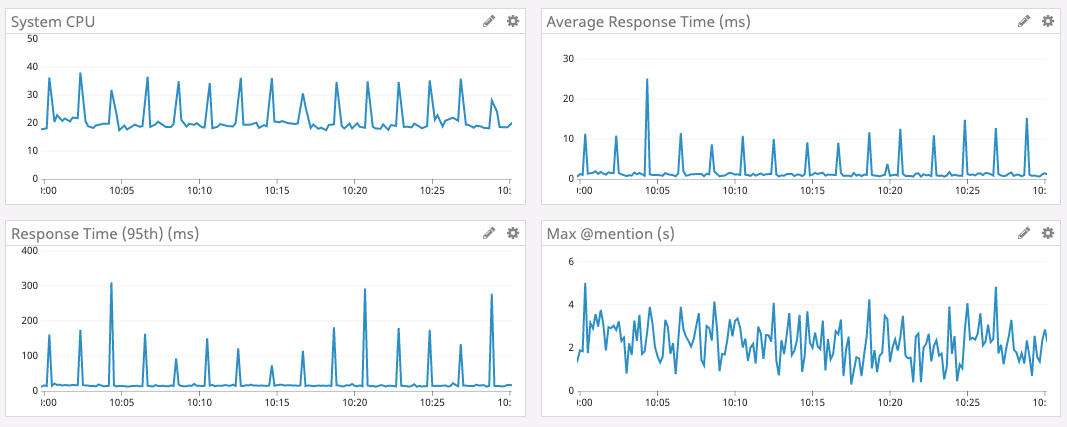
\includegraphics[width=.9\linewidth]{img/gc-impact.png}
\end{center}
\end{frame}
\section{\texttt{Dispose pattern}}
\label{sec:org901ac17}
\begin{frame}[label={sec:orge68c88a},fragile]{\texttt{Dispose pattern}\footnote{\url{https://docs.microsoft.com/en-us/dotnet/standard/garbage-collection/implementing-dispose}\label{orgb023fa7}}}
 \begin{itemize}
\item Este folosit pentru a dealoca memoria resurselor gestionate automat.
\item Este o implementare a metodei \texttt{System.IDisposable.Dispose()}
\end{itemize}
\end{frame}
\begin{frame}[label={sec:org28e28c9},fragile]{\texttt{IDisposable}}
 \begin{verbatim}
public interface IDisposable
{
    void Dispose();
}
\end{verbatim}
\end{frame}
\begin{frame}[label={sec:orgd236052},fragile]{\texttt{Dispose pattern}\textsuperscript{\ref{orgb023fa7}}}
 \begin{verbatim}
public void Dispose()
{
    Dispose(true);
    GC.SuppresFinalize(this);
}
\end{verbatim}
\end{frame}
\begin{frame}[label={sec:orgd27e1f9},fragile]{\texttt{Dispose pattern}\textsuperscript{\ref{orgb023fa7}}}
 \begin{verbatim}
protected virtual void Dispose(bool disposing)
{
    if(this.disposed)
	return;

    if(disposing)
    {
	// Dispose managed resources
    }

    // Dispose unmanaged resources
    this.disposed = true;
}
\end{verbatim}
\end{frame}
\begin{frame}[label={sec:org464bbd7},fragile]{\texttt{Dispose pattern}\textsuperscript{\ref{orgb023fa7}}}
 \begin{verbatim}
~DisposableResource()
{
    Dispose(false);
}
\end{verbatim}
\end{frame}
\section{Cum utilizăm obiecte \texttt{IDisposable}}
\label{sec:org5e8cddd}
\begin{frame}[label={sec:org606ec02},fragile]{Cum utilizăm obiecte \texttt{IDisposable}}
 \begin{itemize}
\item Obiectele care implementează \texttt{IDisposable} trebuie dealocate prin apelarea metodei \texttt{Dispose()}.
\item Apelarea se poate face în două moduri:
\begin{itemize}
\item Cu instrucțiunea \texttt{using} sau,
\item Într-un block \texttt{try/finally}.
\end{itemize}
\end{itemize}
\end{frame}
\begin{frame}[label={sec:orgac5639f},fragile]{Blocul \texttt{try/finally}}
 \begin{verbatim}
DisposableResource res = null;
try
{
    res = new DisposableResource();
    // Do something with the resource
}
finally
{
    if(res != null) res.Dispose();
}
\end{verbatim}
\end{frame}
\begin{frame}[label={sec:org4713340},fragile]{Instrucțiunea \texttt{using}}
 \begin{itemize}
\item Apelează automat metoda \texttt{Dispose()} la părăsirea contextului curent.
\item Este echivalentă cu blocul \texttt{try/finally}.
\end{itemize}
\vskip 0.3in
\begin{verbatim}
using(var res = new DisposableResource())
{
    // Do something with the resource
}
\end{verbatim}
\end{frame}
\section{Ecosistemul \texttt{NuGet}}
\label{sec:org62f5a03}
\begin{frame}[label={sec:org52e88e1},fragile]{Ce este \texttt{NuGet}?}
 \begin{itemize}
\item Aplicație utilitară pentru integrarea bibliotecilor oferite de terți în soluție/proiect.
\item Facilitează instalarea pachetelor și a pachetelor de care acestea depind.
\item Facilitează ștergerea și actualizarea pachetelor.
\end{itemize}
\end{frame}
\begin{frame}[label={sec:orgffdee22},fragile]{Ce este un \texttt{pachet NuGet}?}
 \begin{itemize}
\item O arhivă cu extensia schimbată din \texttt{.zip} în \texttt{.nupkg}.
\item Conține bibliotecile necesare (fișierele \texttt{.dll}) și metadate.
\end{itemize}
\end{frame}
\begin{frame}[label={sec:org63c7437},fragile]{Pachetele \texttt{NuGet}}
 \begin{itemize}
\item Cele publice se găsesc pe \url{https://www.nuget.org/}.
\item Pentru pachetele private sunt necesare servere dedicate.
\end{itemize}
\end{frame}
\section{Încheiere}
\label{sec:orgba9589e}
\begin{frame}[label={sec:orgc98f7d3},fragile]{Recapitulare --- \texttt{GC}}
 \begin{itemize}
\item Resurse gestionate automat vs resurse gestionate manual,
\item Organizarea în 3 generații,
\item Gestionarea ineficientă a resurselor are impact negativ asupra:
\begin{itemize}
\item experienței utilizatorilor,
\item bugetului.
\end{itemize}
\end{itemize}
\end{frame}
\begin{frame}[label={sec:orgc1a9e77},fragile]{Recapitulare --- \texttt{NuGet}}
 Este indicat să folosim \texttt{NuGet} pentru adăugarea de biblioteci în soluție/proiect.
\end{frame}
\begin{frame}[label={sec:orgba83173}]{Vă mulțumesc}
\begin{center}
Mulțumesc pentru atenție!
\end{center}
\end{frame}
\end{document}